\documentclass[conference,10pt]{IEEEtran}
\usepackage{graphicx,amsmath,amssymb,booktabs,url,xcolor}
\usepackage[hidelinks]{hyperref}
\setlength{\textfloatsep}{6pt plus 2pt minus 2pt}
\setlength{\dbltextfloatsep}{6pt plus 2pt minus 2pt}
\setlength{\abovecaptionskip}{2pt}
\setlength{\abovedisplayskip}{3pt}\setlength{\belowdisplayskip}{3pt}

\begin{document}
\title{Learning to Mine from Pixels with Reinforcement Learning}
\author{\IEEEauthorblockN{Chiranjeevi C (B23MT1013), Dhruv Deshwal (B23MT1017)}
\IEEEauthorblockA{AI Course, Assignment 2 \quad$\cdot$\quad
GitHub: \url{https://github.com/itschiru3301/Mining_Bot-AI_Assignement}}}
\maketitle

% Defined early so that it floats to the top of page 2.
\begin{figure*}[t]
\centering
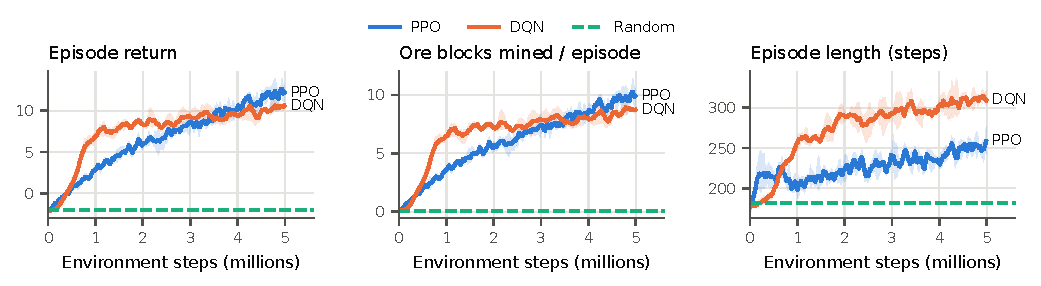
\includegraphics[width=\textwidth]{figures/learning_curves.pdf}
\caption{Training curves (mean of 3 seeds; shading shows the min--max range across seeds; dashed line is the random policy). DQN learns faster at first, but PPO overtakes it after about 3.5M steps. DQN survives longer but mines more slowly.}
\label{fig:curves}
\end{figure*}

\begin{abstract}
Autonomous mining robots must find and extract ore from camera input alone while avoiding hazards. We model this task in Crafter, a procedurally generated world modelled on Minecraft. The agent sees stacked 64$\times$64 RGB frames and its inventory, chooses among six discrete move/mine actions, and is rewarded for every ore block it mines. It pays a small penalty per step and for any damage. A PPO agent written from scratch mines \textbf{10.1 ore blocks per episode} on unseen worlds. That is 31\% more than a Double-DQN baseline (7.7) and over 100$\times$ more than a random policy (0.08). Ablations show that the damage penalty modestly improves survival and that a single-frame observation beats frame stacking (12.8 ores per episode).
\end{abstract}

\section{Problem and Motivation}
Underground mining is dangerous, which makes it a natural target for autonomous robots. A robot must explore unknown terrain, recognise ore from what it sees, tunnel to it and survive hazards. No labelled dataset of ``correct'' mining trajectories exists, but whether ore was extracted and whether the robot was damaged are easy to measure. That makes the problem a good fit for reinforcement learning (RL). Full Minecraft (MineRL~\cite{minerl}) runs at about 60 steps/s, which is too slow for pixel-based RL on a course budget. We therefore use \textbf{Crafter}~\cite{crafter}, which keeps the essential ingredients: egocentric pixels, stone, coal, iron and diamond, lava, zombies, skeletons, a day/night cycle and a new world every episode. It runs at about 1000 steps/s per core. The simulator is used unmodified. The task, reward, vectorised environment, networks, PPO, DQN and evaluation code are our own.

\section{RL Formulation}
\textbf{Environment.} Each episode generates a new 64$\times$64-tile world, and the robot spawns with wood, stone and iron pickaxes. Hunger, thirst and fatigue are disabled because a robot does not eat or sleep. Lava kills instantly. Zombies (on grassland, mostly at night) and skeletons' arrows (in tunnels) deal damage. An episode terminates when health reaches 0 and is truncated after 1000 steps, where we bootstrap from $V(s_T)$.

\textbf{State $\mathcal{S}$.} $s_t=(x_t,u_t)$. $x_t\in\{0..255\}^{12\times64\times64}$ is the last four RGB frames. Each frame shows a 9$\times$7-tile egocentric view plus an inventory strip (Fig.~\ref{fig:frames}). $u_t\in[0,1]^{16}$ is the inventory and vitals vector (health, ores, tools, \dots) divided by its maximum of 9. The state is only partially observable.

\textbf{Actions $\mathcal{A}$.} Six discrete actions: \texttt{noop}, four moves and \texttt{do}. A move also turns the robot to face that direction. \texttt{do} mines the block in front, or attacks a mob there.

\textbf{Reward $\mathcal{R}$.} Let $\Delta n^{k}_t$ be the number of blocks of type $k$ mined at step $t$ (read from uncapped counters, because inventory slots saturate at 9), $\Delta h_t$ the health lost and $d_t$ a death indicator:
\begin{equation}
r_t=\!\!\sum_{k}\! w_k\Delta n^{k}_t - \underbrace{0.001}_{\text{time}} - \underbrace{0.1\,\Delta h_t}_{\text{damage}} - \underbrace{1.0\,d_t}_{\text{destroyed}},
\end{equation}
with $w_{\text{coal}}{=}1$, $w_{\text{iron}}{=}2$, $w_{\text{diamond}}{=}5$, which reflects rarity and value. $w_{\text{stone}}{=}0.02$ is a small shaping term that rewards tunnelling, the robot's way of exploring. The time term rewards speed and the damage and death terms encode safety. $\gamma=0.99$.

\begin{figure}[t]
\centering
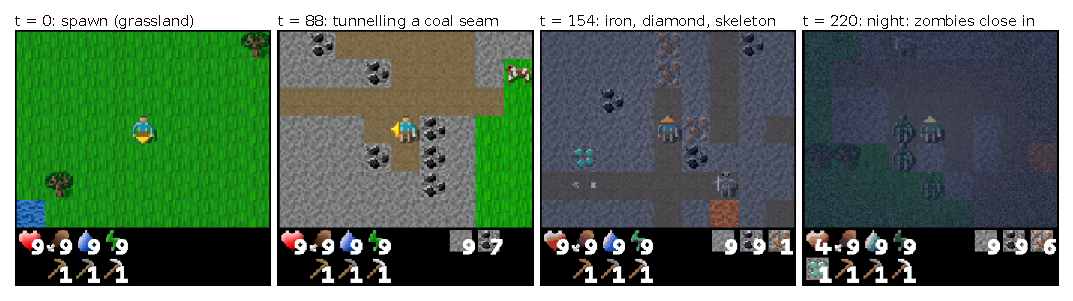
\includegraphics[width=\columnwidth]{figures/agent_frames.pdf}
\caption{An above-average held-out episode of the main PPO agent (return 30.3 vs.\ a mean of 12.7). (a)~Spawn on grassland, (b)~tunnelling a coal seam, (c)~mining iron and a diamond near a skeleton, (d)~worn down by zombies after nightfall.}
\label{fig:frames}
\end{figure}

\section{Algorithms}
\textbf{Network.} The image goes through a 3-layer CNN (32/64/64 filters, kernels 8/4/3, strides 4/2/1) and the inventory through a 64-unit MLP. The outputs are fused into a 512-d feature that feeds the policy and value heads (PPO) or a Q-value head (DQN).

\textbf{PPO (main agent)}~\cite{ppo} maximises
$\mathbb{E}_t[\min(\rho_t\hat A_t,\operatorname{clip}(\rho_t,1{\pm}0.2)\hat A_t)] - 0.5L_V + 0.01\mathcal{H}[\pi]$,
with $\rho_t=\pi_\theta(a_t|s_t)/\pi_{\theta_\text{old}}(a_t|s_t)$ and $\hat A_t$ from GAE ($\lambda{=}0.95$)~\cite{gae}. Each update uses 256-step rollouts from 16 parallel worlds, 4 epochs of 8 minibatches, and Adam at $3{\times}10^{-4}$ with linear decay.

\textbf{DQN (baseline)}~\cite{dqn} uses Double-DQN targets~\cite{ddqn} $y=r+\gamma(1{-}d)\,Q_{\bar\theta}(s',\arg\max_a Q_\theta(s',a))$, a 100k replay buffer, Huber loss, batch size 64, one update per 8 environment steps, a target sync every 10k steps and $\varepsilon$ decaying from 1 to 0.05. \textbf{Random} acts uniformly at random. Each RL agent trains for 5M steps on 3 seeds (PPO about 1.6\,h, DQN about 2.5\,h per seed on one RTX A5000). Evaluation uses 100 episodes per seed in \emph{held-out} worlds.

\section{Results}
\begin{table}[t]
\centering\footnotesize
\caption{Held-out evaluation (mean $\pm$ std over 3 seeds).}
\label{tab:main}
\setlength{\tabcolsep}{3.2pt}
\begin{tabular}{lcccccc}
\toprule
Agent & Return & Coal & Iron & Diamond & Ores/100 st. & Steps \\
\midrule
PPO    & \textbf{12.7}$\pm$0.9 & \textbf{6.85} & \textbf{2.80} & \textbf{0.48} & \textbf{4.46} & 227 \\
DQN    & 9.1$\pm$1.5 & 5.33 & 2.03 & 0.37 & 2.62 & \textbf{296} \\
Random & $-$2.05 & 0.03 & 0.04 & 0.01 & 0.04 & 181 \\
\bottomrule
\end{tabular}
\end{table}

\textbf{Main comparison} (Table~\ref{tab:main}, Fig.~\ref{fig:curves}). Both RL agents learn to leave the grassland, find a deposit and tunnel through it. PPO reaches the highest return and yield, and its lead is largest on the rarer ores (iron +38\%, diamond +30\% over DQN). DQN is more sample-efficient early on, reaching a return of 5 after 0.7--0.8M steps versus 1.4--1.7M for PPO, because it replays each transition many times. It then plateaus around 9--10. DQN also survives longer (296 vs.\ 227 steps) but mines only 2.6 ores per 100 steps against PPO's 4.5. PPO has learned a faster, riskier policy: 16\% of its deaths come from lava, versus 5\% for DQN.

\begin{table}[t]
\centering\footnotesize
\caption{PPO ablations (2 seeds each; main agent 3). All agents are scored with the full reward of Eq.~1.}
\label{tab:abl}
\setlength{\tabcolsep}{3pt}
\begin{tabular}{lccccc}
\toprule
Variant & Frames & Inv. & Dmg.\ pen. & Return & Ores / Steps \\
\midrule
Full PPO (main)      & 4 & \checkmark & \checkmark & 12.7$\pm$0.9 & 10.1 / 227 \\
No damage penalty    & 4 & \checkmark & --         & 12.2$\pm$0.5 & 9.9 / 209 \\
No inventory vector  & 4 & --         & \checkmark & 12.1$\pm$0.5 & 9.5 / 230 \\
\textbf{Single frame}& 1 & \checkmark & \checkmark & \textbf{16.5}$\pm$0.2 & \textbf{12.8} / 255 \\
Single frame, no inv.& 1 & --         & \checkmark & 15.3$\pm$0.9 & 11.9 / 267 \\
\bottomrule
\end{tabular}
\end{table}

\textbf{Ablations} (Table~\ref{tab:abl}). \emph{Reward:} removing the damage and death terms shortens episodes by 8\% and lowers the return slightly. The safety terms help survival, but only modestly, because night-time mobs are hard to escape with this action set. \emph{Observation:} contrary to our proposal's assumption, frame stacking hurts at this budget. A single frame plus the inventory vector is the best agent, mining 12.8 ores per episode (+26\%). Crafter's world is nearly static, so extra frames likely add little motion information while quadrupling the CNN's input. The inventory vector gives a small but consistent gain (+0.6 to +1.1 return), even though the same counts appear in the image.

\textbf{Limitations and future work.} We use only 2--3 seeds per configuration. Almost every episode ends in death soon after the first nightfall (around step 200), because the agent has no weapon and little memory. Natural next steps are a recurrent policy, a \texttt{place\_stone} action for shelter, a survival curriculum and transfer to 3-D MineRL.

\begin{thebibliography}{9}\footnotesize
\bibitem{crafter} D.~Hafner, ``Benchmarking the spectrum of agent capabilities,'' \emph{ICLR}, 2022.
\bibitem{minerl} W.~H.~Guss \emph{et al.}, ``MineRL: A large-scale dataset of Minecraft demonstrations,'' \emph{IJCAI}, 2019.
\bibitem{ppo} J.~Schulman \emph{et al.}, ``Proximal policy optimization algorithms,'' arXiv:1707.06347, 2017.
\bibitem{gae} J.~Schulman \emph{et al.}, ``High-dimensional continuous control using generalized advantage estimation,'' \emph{ICLR}, 2016.
\bibitem{dqn} V.~Mnih \emph{et al.}, ``Human-level control through deep reinforcement learning,'' \emph{Nature}, 2015.
\bibitem{ddqn} H.~van Hasselt, A.~Guez, D.~Silver, ``Deep reinforcement learning with double Q-learning,'' \emph{AAAI}, 2016.
\end{thebibliography}
\end{document}
